\subsection{Distributed SGF FW Experiments}
To test the performance of Algorithm \ref{distributed} we used a distributed network of $M=10$ worker nodes and we
gave them 10 images per class each, for a total of 100 different images each.

The connectivity of the graph describing the distributed setting is represented by the value $\Vert \mathbf{W}- \mathbf{J} \Vert$,
where $\mathbf{J}= \mathbf{11}^T/M$ with $\mathbf{11}^T$ the matrix having all entries set to 1.\\ For the experiments, we created a network
with a connectivity value of 0.438 given by the following adjacecy
matrix:
\[ A =
\begin{pmatrix}
1& 1& 0& 1& 1& 1& 1& 1& 0& 1\\
1& 1& 1& 0& 1& 1& 1& 0& 1& 1\\
0& 1& 1& 1& 1& 1& 0& 1& 1& 1\\
1& 0& 1& 1& 1& 1& 0& 1& 1& 1\\
1& 1& 1& 1& 1& 1& 1& 0& 1& 1\\
1& 1& 1& 1& 1& 1& 1& 1& 1& 0\\
1& 1& 0& 0& 1& 1& 1& 1& 1& 1\\
1& 0& 1& 1& 0& 1& 1& 1& 1& 1\\
0& 1& 1& 1& 1& 1& 1& 1& 1& 1\\
1& 1& 1& 1& 1& 0& 1& 1& 1& 1
\end{pmatrix}
.\]
Since each node is connected to itself, the diagonal of the matrix A is filled with ones.
Furthermore, we computed the I-RDSA approximated gradient scheme along $m=15$ directions and we tested the algorithm for $T=20$, $T=50$ and $T=100$ queries.

In Figure \ref{fig:perturbations} we can see the universal adversarial perturbations produced by Algorithm \ref{distributed}
for different values of T. It's clear that the three perturbations are very similar to each other and all of them present a quite evident 3-shape.
\begin{figure}[h]
	\centering
	\begin{subfigure}[b]{0.15\textwidth}
		\centering
		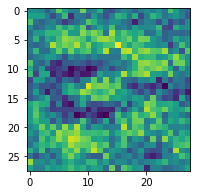
\includegraphics[width=2.3cm]{T20_final_distr.png}
		\caption{}
		\label{fig:distributed_perturbation_20}
	\end{subfigure}
	\hfill
	\begin{subfigure}[b]{0.15\textwidth}
		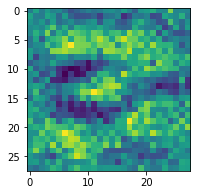
\includegraphics[width=2.3cm]{T50_final_distr.png}
		\caption{}
		\label{fig:variance-distributed_perturbation_50}
	\end{subfigure}
	\hfill
	\begin{subfigure}[b]{0.15\textwidth}
		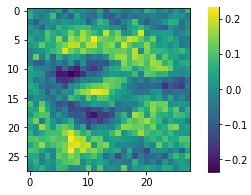
\includegraphics[width=2.9cm]{T100_final_bar.png}
		\caption{}
		\label{fig:distributed_perturbation_100}
	\end{subfigure}
	\caption{{\small Perturbations generated by the Distributed SGF FW algorithm with different numbers of queries: (a) T=20, (b) T=50, (c) T=100.}}
	\label{fig:perturbations}
\end{figure}


In Figure \ref{fig:distributed} is represented the perturbation of Figure \ref{fig:perturbations} (c) applied on an image from class 2.

\begin{figure}[htbp]
	\centering
	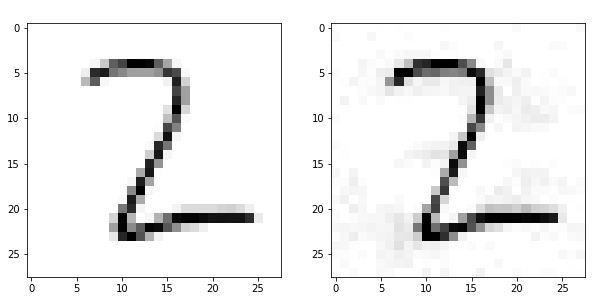
\includegraphics[width=6cm]{image_pertub_T100_final_distr.png}
	\caption{{\small Image belonging to class 2 but classified as 3 by using the adversarial perturbation in Figure \ref{fig:perturbations} (c) generated by the Distributed SGF FW method.}}
	\label{fig:distributed}
\end{figure}
Although we can still recognize the 3-shape pattern in the
perturbation, it is much smoother compared to the perturbation in Figure \ref{fig:decentralized_perturbations} (c) computed by the Decentralized
SGF FW algorithm. Nevertheless, it is strong enough to fool the classifier and lead it to a wrong prediction.

The Table \ref{tab:distributed} displays the values of accuracy reached by the LeNet-5 classifier on perturbed images, generated using the results of Algorithm \ref{decentralized} with different amounts of queries.\\
\begin{table}[htbp]
	\begin{center}
		\begin{adjustwidth}{-.6cm}{}
			\begin{tabular}{c|ccc}
				\textbf{Attack} &          20 \textbf{queries} &      50 \textbf{queries} &     100 \textbf{queries} \\
				\midrule
				{\small Distributed SGF FW}     &   73.47\% &    74.62\% &       75.84\% \\
			\end{tabular}
		\end{adjustwidth}
	\end{center}
	\caption{{\small Summary of $\ell_\infty$ Universal Adversarial Perturbation with $\varepsilon$=0.25. MNIST attacks using Distributed SGF FW. The entries of the table represent the accuracies of LeNet-5 for the three different attacks.}}
	\label{tab:distributed}
\end{table}

We can see that there's no significant
difference among the accuracy values corresponding to different number of queries. What we can notice is that the
perturbation becomes slightly less effective in fooling the classifier, as long as we increase the number of queries.